% Options for packages loaded elsewhere
\PassOptionsToPackage{unicode=true}{hyperref}
\PassOptionsToPackage{hyphens}{url}
%
\documentclass[
]{article}
\usepackage{lmodern}
\usepackage{amssymb,amsmath}
\usepackage{ifxetex,ifluatex}
\ifnum 0\ifxetex 1\fi\ifluatex 1\fi=0 % if pdftex
  \usepackage[T1]{fontenc}
  \usepackage[utf8]{inputenc}
  \usepackage{textcomp} % provides euro and other symbols
\else % if luatex or xelatex
  \usepackage{unicode-math}
  \defaultfontfeatures{Scale=MatchLowercase}
  \defaultfontfeatures[\rmfamily]{Ligatures=TeX,Scale=1}
\fi
% Use upquote if available, for straight quotes in verbatim environments
\IfFileExists{upquote.sty}{\usepackage{upquote}}{}
\IfFileExists{microtype.sty}{% use microtype if available
  \usepackage[]{microtype}
  \UseMicrotypeSet[protrusion]{basicmath} % disable protrusion for tt fonts
}{}
\makeatletter
\@ifundefined{KOMAClassName}{% if non-KOMA class
  \IfFileExists{parskip.sty}{%
    \usepackage{parskip}
  }{% else
    \setlength{\parindent}{0pt}
    \setlength{\parskip}{6pt plus 2pt minus 1pt}}
}{% if KOMA class
  \KOMAoptions{parskip=half}}
\makeatother
\usepackage{xcolor}
\IfFileExists{xurl.sty}{\usepackage{xurl}}{} % add URL line breaks if available
\IfFileExists{bookmark.sty}{\usepackage{bookmark}}{\usepackage{hyperref}}
\hypersetup{
  pdftitle={Gibss-sampling-Activity-Solution},
  hidelinks,
}
\urlstyle{same} % disable monospaced font for URLs
\usepackage[margin=1in]{geometry}
\usepackage{color}
\usepackage{fancyvrb}
\newcommand{\VerbBar}{|}
\newcommand{\VERB}{\Verb[commandchars=\\\{\}]}
\DefineVerbatimEnvironment{Highlighting}{Verbatim}{commandchars=\\\{\}}
% Add ',fontsize=\small' for more characters per line
\usepackage{framed}
\definecolor{shadecolor}{RGB}{248,248,248}
\newenvironment{Shaded}{\begin{snugshade}}{\end{snugshade}}
\newcommand{\AlertTok}[1]{\textcolor[rgb]{0.94,0.16,0.16}{#1}}
\newcommand{\AnnotationTok}[1]{\textcolor[rgb]{0.56,0.35,0.01}{\textbf{\textit{#1}}}}
\newcommand{\AttributeTok}[1]{\textcolor[rgb]{0.77,0.63,0.00}{#1}}
\newcommand{\BaseNTok}[1]{\textcolor[rgb]{0.00,0.00,0.81}{#1}}
\newcommand{\BuiltInTok}[1]{#1}
\newcommand{\CharTok}[1]{\textcolor[rgb]{0.31,0.60,0.02}{#1}}
\newcommand{\CommentTok}[1]{\textcolor[rgb]{0.56,0.35,0.01}{\textit{#1}}}
\newcommand{\CommentVarTok}[1]{\textcolor[rgb]{0.56,0.35,0.01}{\textbf{\textit{#1}}}}
\newcommand{\ConstantTok}[1]{\textcolor[rgb]{0.00,0.00,0.00}{#1}}
\newcommand{\ControlFlowTok}[1]{\textcolor[rgb]{0.13,0.29,0.53}{\textbf{#1}}}
\newcommand{\DataTypeTok}[1]{\textcolor[rgb]{0.13,0.29,0.53}{#1}}
\newcommand{\DecValTok}[1]{\textcolor[rgb]{0.00,0.00,0.81}{#1}}
\newcommand{\DocumentationTok}[1]{\textcolor[rgb]{0.56,0.35,0.01}{\textbf{\textit{#1}}}}
\newcommand{\ErrorTok}[1]{\textcolor[rgb]{0.64,0.00,0.00}{\textbf{#1}}}
\newcommand{\ExtensionTok}[1]{#1}
\newcommand{\FloatTok}[1]{\textcolor[rgb]{0.00,0.00,0.81}{#1}}
\newcommand{\FunctionTok}[1]{\textcolor[rgb]{0.00,0.00,0.00}{#1}}
\newcommand{\ImportTok}[1]{#1}
\newcommand{\InformationTok}[1]{\textcolor[rgb]{0.56,0.35,0.01}{\textbf{\textit{#1}}}}
\newcommand{\KeywordTok}[1]{\textcolor[rgb]{0.13,0.29,0.53}{\textbf{#1}}}
\newcommand{\NormalTok}[1]{#1}
\newcommand{\OperatorTok}[1]{\textcolor[rgb]{0.81,0.36,0.00}{\textbf{#1}}}
\newcommand{\OtherTok}[1]{\textcolor[rgb]{0.56,0.35,0.01}{#1}}
\newcommand{\PreprocessorTok}[1]{\textcolor[rgb]{0.56,0.35,0.01}{\textit{#1}}}
\newcommand{\RegionMarkerTok}[1]{#1}
\newcommand{\SpecialCharTok}[1]{\textcolor[rgb]{0.00,0.00,0.00}{#1}}
\newcommand{\SpecialStringTok}[1]{\textcolor[rgb]{0.31,0.60,0.02}{#1}}
\newcommand{\StringTok}[1]{\textcolor[rgb]{0.31,0.60,0.02}{#1}}
\newcommand{\VariableTok}[1]{\textcolor[rgb]{0.00,0.00,0.00}{#1}}
\newcommand{\VerbatimStringTok}[1]{\textcolor[rgb]{0.31,0.60,0.02}{#1}}
\newcommand{\WarningTok}[1]{\textcolor[rgb]{0.56,0.35,0.01}{\textbf{\textit{#1}}}}
\usepackage{graphicx,grffile}
\makeatletter
\def\maxwidth{\ifdim\Gin@nat@width>\linewidth\linewidth\else\Gin@nat@width\fi}
\def\maxheight{\ifdim\Gin@nat@height>\textheight\textheight\else\Gin@nat@height\fi}
\makeatother
% Scale images if necessary, so that they will not overflow the page
% margins by default, and it is still possible to overwrite the defaults
% using explicit options in \includegraphics[width, height, ...]{}
\setkeys{Gin}{width=\maxwidth,height=\maxheight,keepaspectratio}
\setlength{\emergencystretch}{3em} % prevent overfull lines
\providecommand{\tightlist}{%
  \setlength{\itemsep}{0pt}\setlength{\parskip}{0pt}}
\setcounter{secnumdepth}{-\maxdimen} % remove section numbering
% Redefines (sub)paragraphs to behave more like sections
\ifx\paragraph\undefined\else
  \let\oldparagraph\paragraph
  \renewcommand{\paragraph}[1]{\oldparagraph{#1}\mbox{}}
\fi
\ifx\subparagraph\undefined\else
  \let\oldsubparagraph\subparagraph
  \renewcommand{\subparagraph}[1]{\oldsubparagraph{#1}\mbox{}}
\fi

% Set default figure placement to htbp
\makeatletter
\def\fps@figure{htbp}
\makeatother


\title{Gibss-sampling-Activity-Solution}
\author{}
\date{\vspace{-2.5em}}

\begin{document}
\maketitle

\hypertarget{instructions}{%
\section{Instructions}\label{instructions}}

\begin{enumerate}
\def\labelenumi{\arabic{enumi}.}
\item
  Download this \texttt{.Rmd} file and open it in RStudio.
\item
  Update the author name and date.
\item
  Answer the questions below, using LaTeX within R Markdown to type up
  your answers.
\item
  When you finish, \texttt{Knit\ to\ PDF}.
\end{enumerate}

\hypertarget{markov-chains}{%
\section{Markov Chains}\label{markov-chains}}

First we will implement a Markov chain. We will conduct the MCMC
simulation using the rstan package (Guo and Weber 2020). There are two
essential steps to all rstan analyses, first we define the Bayesian
model structure and then simulate the posterior. We will use a generical
Beta-Binomial example:

\[Y\mid \pi \sim Bin(10,\pi)\] \[\pi \sim Beta(2,2)\]

Where Y is the number of successes in 10 independent trials. Each trial
has a probability of success \(\pi\) where our prior for \(\pi\) is
captured by a \(Beta(2,2)\) model. If we observe 9 successes we have an
updated posterior model of \(\pi\) with distribution \(Beta(11,3)\).
Don't worry about how we arrived to this posterior for the moment being.
Keep in mind our goal is to run an MCMC algorithm to produce an
approximate sample from the Beta-binomial posterior \(Beta(11,3)\).

\hypertarget{this-plot-represents-our-prior-beliefs}{%
\subsubsection{This plot represents our prior
beliefs}\label{this-plot-represents-our-prior-beliefs}}

\begin{Shaded}
\begin{Highlighting}[]
\KeywordTok{plot_beta}\NormalTok{(}\DecValTok{2}\NormalTok{,}\DecValTok{2}\NormalTok{)}
\end{Highlighting}
\end{Shaded}

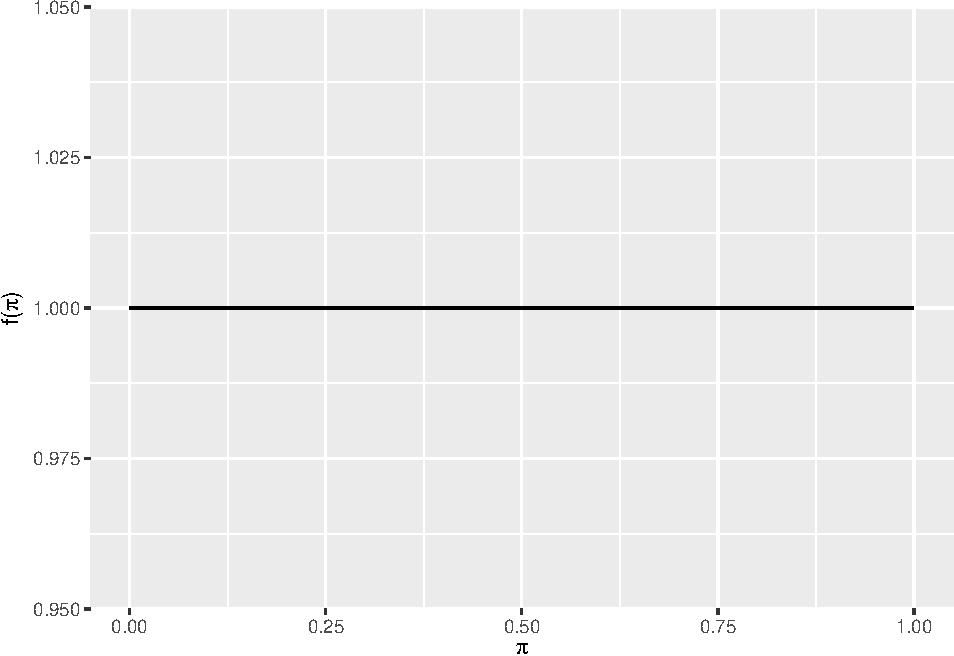
\includegraphics[width=0.5\linewidth]{Gibbs-sampling-solutions_files/figure-latex/unnamed-chunk-2-1}

\hypertarget{this-plot-shows-our-likelihood-based-on-our-two-data-points}{%
\subsubsection{This plot shows our likelihood based on our two data
points}\label{this-plot-shows-our-likelihood-based-on-our-two-data-points}}

\begin{Shaded}
\begin{Highlighting}[]
\KeywordTok{plot_binomial_likelihood}\NormalTok{(}\DataTypeTok{y =} \DecValTok{9}\NormalTok{,}\DataTypeTok{n =} \DecValTok{10}\NormalTok{)}
\end{Highlighting}
\end{Shaded}

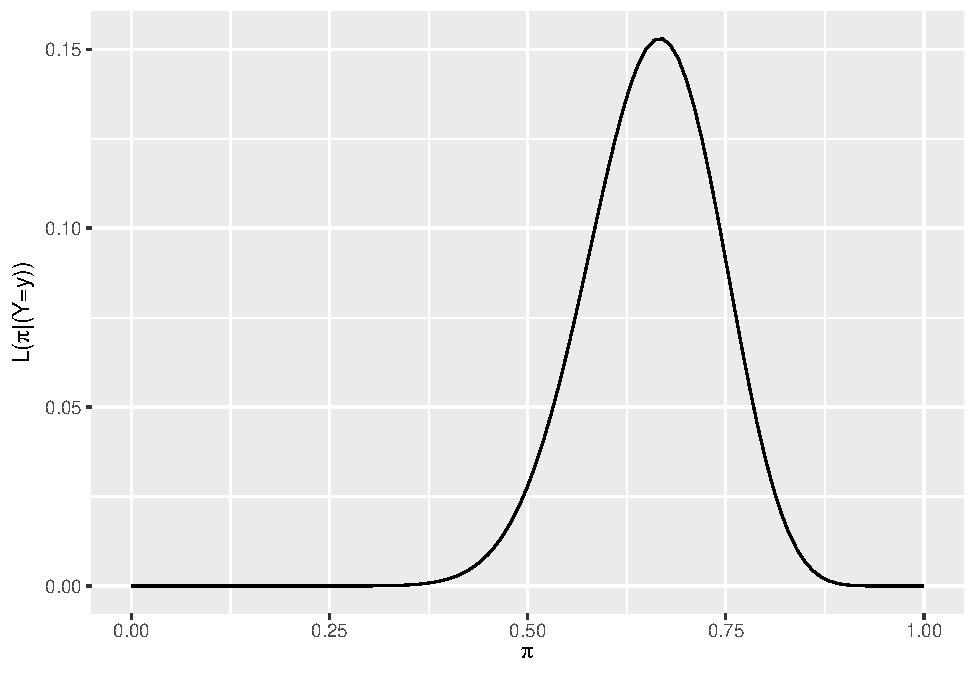
\includegraphics[width=0.5\linewidth]{Gibbs-sampling-solutions_files/figure-latex/unnamed-chunk-3-1}

\hypertarget{step-1-define-the-model}{%
\subsubsection{STEP 1: DEFINE the model}\label{step-1-define-the-model}}

Observe there are 3 different elements of this code. You don't need to
change anything, but we encourage you to identify the prior, posterior
and parameters of the model in the code.

\emph{Data}: Y is the observed number of success trials. We specify that
Y is between 10 and 0.

\emph{Parameters}: The model depends on \(\pi\), therefore we must
specify that \(\pi\) can be any real number from 0 to 1.

\emph{Model}: We need to specify the model for the data and the model
for the prior.

\begin{Shaded}
\begin{Highlighting}[]
\CommentTok{# STEP 1: DEFINE the model}
\NormalTok{bb_model <-}\StringTok{ "}
\StringTok{  data \{}
\StringTok{    int<lower = 0, upper = 10> Y;}
\StringTok{  \}}
\StringTok{  parameters \{}
\StringTok{    real<lower = 0, upper = 1> pi;}
\StringTok{  \}}
\StringTok{  model \{}
\StringTok{    Y ~ binomial(10, pi);}
\StringTok{    pi ~ beta(2, 2);}
\StringTok{  \}}
\StringTok{"}
\end{Highlighting}
\end{Shaded}

\hypertarget{step-2-simulate-the-posterior}{%
\subsubsection{STEP 2: Simulate the
posterior}\label{step-2-simulate-the-posterior}}

We simulate the posterior using the stan() function. This function
designs and runs an MCMC algorithm to produce an approximate sample from
the Beta-Binomial posterior.

The \emph{model\_code} argument requires a string that defines the
model, which we created in the previous step.

The \emph{data} argument requires a list of observed data.

The \emph{chains} argument specifies how many parallel Markov Chains we
are running. Since we are running four chains we will have four \(\pi\)
values.

The \emph{iter} argument specifies the number of iterations or length
for each chain. The first half of this iterations are thrown out as
``burn in'' samples (samples that we use to calibrate our model).

We utilize the \emph{seed} argument within the stan() function to keep
our random results constant.

\begin{Shaded}
\begin{Highlighting}[]
\NormalTok{bb_sim <-}\StringTok{ }\KeywordTok{stan}\NormalTok{(}\DataTypeTok{model_code =}\NormalTok{ bb_model, }\CommentTok{#model_code argument}
               \DataTypeTok{data =} \KeywordTok{list}\NormalTok{(}\DataTypeTok{Y =} \DecValTok{9}\NormalTok{),  }\CommentTok{# data argument}
               \DataTypeTok{chains =} \DecValTok{4}\NormalTok{, }\CommentTok{#we are running four chains}
               \DataTypeTok{iter =} \DecValTok{5000}\OperatorTok{*}\DecValTok{2}\NormalTok{, }\CommentTok{#number of iterations or length for each chain}
               \DataTypeTok{seed =} \DecValTok{84735}\NormalTok{) }\CommentTok{#keep our random results constant}
\end{Highlighting}
\end{Shaded}

\begin{verbatim}
## 
## SAMPLING FOR MODEL '552853291e881827cbfc36dff498b1a9' NOW (CHAIN 1).
## Chain 1: 
## Chain 1: Gradient evaluation took 0 seconds
## Chain 1: 1000 transitions using 10 leapfrog steps per transition would take 0 seconds.
## Chain 1: Adjust your expectations accordingly!
## Chain 1: 
## Chain 1: 
## Chain 1: Iteration:    1 / 10000 [  0%]  (Warmup)
## Chain 1: Iteration: 1000 / 10000 [ 10%]  (Warmup)
## Chain 1: Iteration: 2000 / 10000 [ 20%]  (Warmup)
## Chain 1: Iteration: 3000 / 10000 [ 30%]  (Warmup)
## Chain 1: Iteration: 4000 / 10000 [ 40%]  (Warmup)
## Chain 1: Iteration: 5000 / 10000 [ 50%]  (Warmup)
## Chain 1: Iteration: 5001 / 10000 [ 50%]  (Sampling)
## Chain 1: Iteration: 6000 / 10000 [ 60%]  (Sampling)
## Chain 1: Iteration: 7000 / 10000 [ 70%]  (Sampling)
## Chain 1: Iteration: 8000 / 10000 [ 80%]  (Sampling)
## Chain 1: Iteration: 9000 / 10000 [ 90%]  (Sampling)
## Chain 1: Iteration: 10000 / 10000 [100%]  (Sampling)
## Chain 1: 
## Chain 1:  Elapsed Time: 0.046 seconds (Warm-up)
## Chain 1:                0.048 seconds (Sampling)
## Chain 1:                0.094 seconds (Total)
## Chain 1: 
## 
## SAMPLING FOR MODEL '552853291e881827cbfc36dff498b1a9' NOW (CHAIN 2).
## Chain 2: 
## Chain 2: Gradient evaluation took 0 seconds
## Chain 2: 1000 transitions using 10 leapfrog steps per transition would take 0 seconds.
## Chain 2: Adjust your expectations accordingly!
## Chain 2: 
## Chain 2: 
## Chain 2: Iteration:    1 / 10000 [  0%]  (Warmup)
## Chain 2: Iteration: 1000 / 10000 [ 10%]  (Warmup)
## Chain 2: Iteration: 2000 / 10000 [ 20%]  (Warmup)
## Chain 2: Iteration: 3000 / 10000 [ 30%]  (Warmup)
## Chain 2: Iteration: 4000 / 10000 [ 40%]  (Warmup)
## Chain 2: Iteration: 5000 / 10000 [ 50%]  (Warmup)
## Chain 2: Iteration: 5001 / 10000 [ 50%]  (Sampling)
## Chain 2: Iteration: 6000 / 10000 [ 60%]  (Sampling)
## Chain 2: Iteration: 7000 / 10000 [ 70%]  (Sampling)
## Chain 2: Iteration: 8000 / 10000 [ 80%]  (Sampling)
## Chain 2: Iteration: 9000 / 10000 [ 90%]  (Sampling)
## Chain 2: Iteration: 10000 / 10000 [100%]  (Sampling)
## Chain 2: 
## Chain 2:  Elapsed Time: 0.049 seconds (Warm-up)
## Chain 2:                0.047 seconds (Sampling)
## Chain 2:                0.096 seconds (Total)
## Chain 2: 
## 
## SAMPLING FOR MODEL '552853291e881827cbfc36dff498b1a9' NOW (CHAIN 3).
## Chain 3: 
## Chain 3: Gradient evaluation took 0 seconds
## Chain 3: 1000 transitions using 10 leapfrog steps per transition would take 0 seconds.
## Chain 3: Adjust your expectations accordingly!
## Chain 3: 
## Chain 3: 
## Chain 3: Iteration:    1 / 10000 [  0%]  (Warmup)
## Chain 3: Iteration: 1000 / 10000 [ 10%]  (Warmup)
## Chain 3: Iteration: 2000 / 10000 [ 20%]  (Warmup)
## Chain 3: Iteration: 3000 / 10000 [ 30%]  (Warmup)
## Chain 3: Iteration: 4000 / 10000 [ 40%]  (Warmup)
## Chain 3: Iteration: 5000 / 10000 [ 50%]  (Warmup)
## Chain 3: Iteration: 5001 / 10000 [ 50%]  (Sampling)
## Chain 3: Iteration: 6000 / 10000 [ 60%]  (Sampling)
## Chain 3: Iteration: 7000 / 10000 [ 70%]  (Sampling)
## Chain 3: Iteration: 8000 / 10000 [ 80%]  (Sampling)
## Chain 3: Iteration: 9000 / 10000 [ 90%]  (Sampling)
## Chain 3: Iteration: 10000 / 10000 [100%]  (Sampling)
## Chain 3: 
## Chain 3:  Elapsed Time: 0.051 seconds (Warm-up)
## Chain 3:                0.055 seconds (Sampling)
## Chain 3:                0.106 seconds (Total)
## Chain 3: 
## 
## SAMPLING FOR MODEL '552853291e881827cbfc36dff498b1a9' NOW (CHAIN 4).
## Chain 4: 
## Chain 4: Gradient evaluation took 0 seconds
## Chain 4: 1000 transitions using 10 leapfrog steps per transition would take 0 seconds.
## Chain 4: Adjust your expectations accordingly!
## Chain 4: 
## Chain 4: 
## Chain 4: Iteration:    1 / 10000 [  0%]  (Warmup)
## Chain 4: Iteration: 1000 / 10000 [ 10%]  (Warmup)
## Chain 4: Iteration: 2000 / 10000 [ 20%]  (Warmup)
## Chain 4: Iteration: 3000 / 10000 [ 30%]  (Warmup)
## Chain 4: Iteration: 4000 / 10000 [ 40%]  (Warmup)
## Chain 4: Iteration: 5000 / 10000 [ 50%]  (Warmup)
## Chain 4: Iteration: 5001 / 10000 [ 50%]  (Sampling)
## Chain 4: Iteration: 6000 / 10000 [ 60%]  (Sampling)
## Chain 4: Iteration: 7000 / 10000 [ 70%]  (Sampling)
## Chain 4: Iteration: 8000 / 10000 [ 80%]  (Sampling)
## Chain 4: Iteration: 9000 / 10000 [ 90%]  (Sampling)
## Chain 4: Iteration: 10000 / 10000 [100%]  (Sampling)
## Chain 4: 
## Chain 4:  Elapsed Time: 0.051 seconds (Warm-up)
## Chain 4:                0.047 seconds (Sampling)
## Chain 4:                0.098 seconds (Total)
## Chain 4:
\end{verbatim}

As you can see in Figure 1, when observing the distribution of the
sampled \(\pi\) values we approximate the target Beta(11,3) posterior
model of \(\pi\). The target pdf superimposed to our simulated model.
Excellent! Now you know how to approximate a posterior using Markov
Chains (Alicia A. Johnson 2022).

\begin{Shaded}
\begin{Highlighting}[]
\CommentTok{# Histogram of the Markov chain values}
\KeywordTok{mcmc_hist}\NormalTok{(bb_sim, }\DataTypeTok{pars =} \StringTok{"pi"}\NormalTok{) }\OperatorTok{+}\StringTok{ }
\StringTok{  }\KeywordTok{yaxis_text}\NormalTok{(}\OtherTok{TRUE}\NormalTok{) }\OperatorTok{+}\StringTok{ }
\StringTok{  }\KeywordTok{ylab}\NormalTok{(}\StringTok{"count"}\NormalTok{)}
\end{Highlighting}
\end{Shaded}

\begin{verbatim}
## `stat_bin()` using `bins = 30`. Pick better value with `binwidth`.
\end{verbatim}

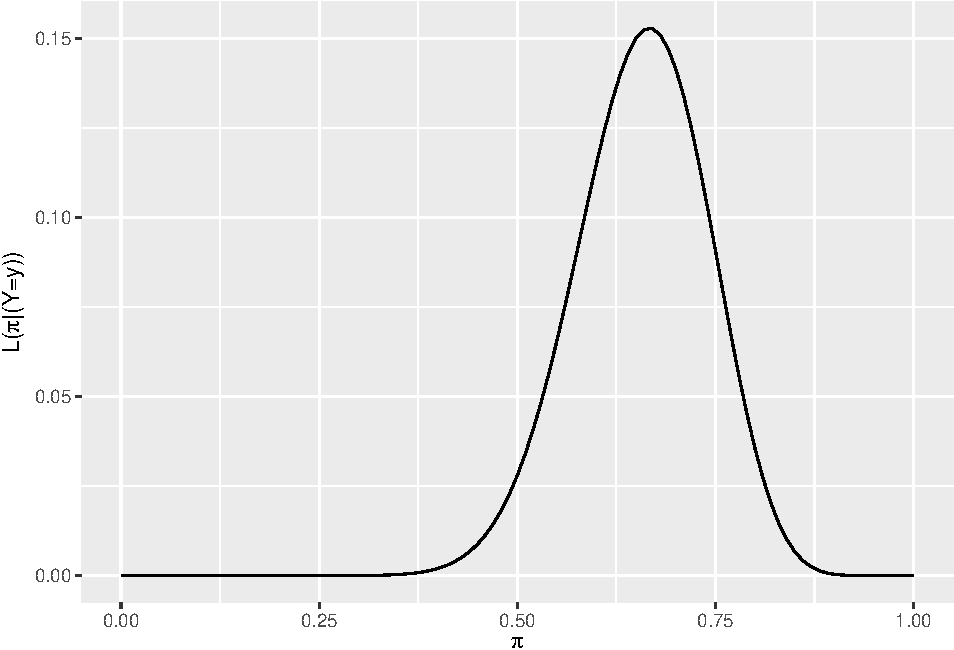
\includegraphics[width=0.5\linewidth]{Gibbs-sampling-solutions_files/figure-latex/unnamed-chunk-6-1}

\begin{Shaded}
\begin{Highlighting}[]
\CommentTok{# Density plot of the Markov chain values}
\NormalTok{p =}\StringTok{ }\KeywordTok{seq}\NormalTok{(}\DecValTok{0}\NormalTok{, }\DecValTok{1}\NormalTok{, }\DataTypeTok{length=}\DecValTok{100}\NormalTok{)}
\KeywordTok{mcmc_dens}\NormalTok{(bb_sim, }\DataTypeTok{pars =} \StringTok{"pi"}\NormalTok{) }\OperatorTok{+}\StringTok{ }
\StringTok{  }\KeywordTok{yaxis_text}\NormalTok{(}\OtherTok{TRUE}\NormalTok{) }\OperatorTok{+}\StringTok{ }
\StringTok{  }\KeywordTok{ylab}\NormalTok{(}\StringTok{"density"}\NormalTok{)}\OperatorTok{+}
\StringTok{  }\KeywordTok{stat_function}\NormalTok{(}\DataTypeTok{fun =}\NormalTok{ dbeta, }\DataTypeTok{args =} \KeywordTok{list}\NormalTok{(}\DecValTok{11}\NormalTok{, }\DecValTok{3}\NormalTok{)) }
\end{Highlighting}
\end{Shaded}

\includegraphics[width=0.5\linewidth]{Gibbs-sampling-solutions_files/figure-latex/unnamed-chunk-6-2}

\hypertarget{gibbs-sampling}{%
\section{Gibbs Sampling}\label{gibbs-sampling}}

Suppose we have data from a normal distribution where both the mean
\textbf{and} variance are unknown. For convenience, we'll parameterize
this model in terms of the \emph{precision}
\(\gamma = \frac{1}{\sigma^2}\) instead of the variance \(\sigma^2\).

\[Y \mid \mu, \gamma \sim N\left(\mu, \frac{1}{\gamma}\right)\]

Suppose we put the following \emph{independent} priors on the mean
\(\mu\) and precision \(\gamma\):

\[\mu \sim N(m, v)\]

\[\gamma \sim \text{Gamma}(a,b)\]

\begin{enumerate}
\def\labelenumi{\arabic{enumi}.}
\tightlist
\item
  Write down the joint posterior distribution for \(\mu, \gamma\). Does
  this look like a recognizable probability distribution?
\end{enumerate}

\textbf{ANSWER:}

\[
\begin{aligned}
g(\mu,\gamma \mid y) & \propto f(y \mid \mu, \gamma) f(\mu, \gamma) \\
& = \dots \\
& =\gamma^{\frac{1}{2} + a - 1}e^{-\frac{1}{2}\gamma(y - \mu)^2 + -\frac{1}{2v}(\mu - m)^2 -b\gamma} \\
& = \gamma^{\frac{1}{2} + a - 1}e^{-\frac{1}{2}\left[\gamma(y - \mu)^2 + \frac{1}{v}(\mu - m)^2 + 2b\gamma\right]} \\
& = \gamma^{\frac{1}{2} + a - 1}e^{-\frac{1}{2}\left[\gamma y^2 - 2\mu y \gamma + \gamma \mu^2 + \mu^2 / v - 2m \mu / v + m^2 / v + 2 b \gamma\right]} \\
& = \gamma^{\frac{1}{2} + a - 1}e^{-\frac{1}{2}\left[\gamma (y^2 + 2b) - 2\mu (y \gamma + m/v) + \mu^2(\gamma  + 1 / v)  + m^2 / v \right]} \\
& \propto \gamma^{\frac{1}{2}+a-1}e^{-\frac{1}{2}\left[\gamma(y^2 + 2b) - 2\mu(y\gamma + \frac{m}{v}) + \mu^2(\frac{1}{v}+ \gamma) \right]} \\
\end{aligned}
\]

You should have answered ``no'' to Question 1, meaning that we can't use
our usual techniques here to find Bayes estimators for \(\mu\) or
\(\gamma\) since we don't have a recognizable posterior distribution.
Instead, we'll use a computational technique known as \emph{Gibbs
Sampling} to generate samples from this posterior distribution. Gibbs
Sampling is particularly useful when we have more than one parameter,
and the basic idea involves reducing our problem to a series of
calculations involving one parameter at a time. In order to perform
Gibbs Sampling, we need to find the conditional distributions
\[g(\mu \mid y, \gamma) \propto f(y \mid \mu, \gamma)f(\mu)\]
\[g(\gamma \mid y, \mu) \propto f(y \mid \mu,\gamma)f(\gamma)\] We will
use these conditional distributions to sample from the joint posterior
\(g(\mu, \gamma \mid y)\) according to the following algorithm:

\begin{quote}
\begin{enumerate}
\def\labelenumi{(\arabic{enumi})}
\tightlist
\item
  Start with initial values \(\mu^{(0)}, \gamma^{(0)}\).
\end{enumerate}
\end{quote}

\begin{quote}
\begin{enumerate}
\def\labelenumi{(\arabic{enumi})}
\setcounter{enumi}{1}
\tightlist
\item
  Sample \(\mu^{(t+1)} \sim g(\mu \mid y, \gamma = \gamma^{(t)})\).
\end{enumerate}
\end{quote}

\begin{quote}
\begin{enumerate}
\def\labelenumi{(\arabic{enumi})}
\setcounter{enumi}{2}
\tightlist
\item
  Sample \(\gamma^{(t+1)} \sim g(\gamma \mid y, \mu = \mu^{(t+1)})\).
\end{enumerate}
\end{quote}

\begin{quote}
\begin{enumerate}
\def\labelenumi{(\arabic{enumi})}
\setcounter{enumi}{3}
\tightlist
\item
  Repeat many times.
\end{enumerate}
\end{quote}

It turns out that the resulting
\(\mu^{(0)}, \mu^{(1)}, \dots, \mu^{(N)}\) and
\(\gamma^{(0)}, \gamma^{(1)}, \dots, \gamma^{(N)}\) are samples from the
joint posterior distribution \(g(\mu, \gamma \mid Y)\), and we can use
these sampled values to estimate quantities such as the posterior mean
of each parameter
\(\hat{E}(\mu \mid y) = \frac{1}{N}\sum_{i=1}^N \mu^{(i)}, \ \ \hat{E}(\gamma \mid y) = \frac{1}{N}\sum_{i=1}^N \gamma^{(i)}\).
Note that in practice we typically remove the initial iterations, known
as the ``burn-in'' period: e.g.,
\(\hat{E}(\mu \mid y) = \frac{1}{N-B}\sum_{i=B}^N \mu^{(i)}\).

\begin{enumerate}
\def\labelenumi{\arabic{enumi}.}
\setcounter{enumi}{1}
\tightlist
\item
  Show that the conditional distributions
  \(g(\mu \mid y, \gamma), g(\gamma \mid y, \mu)\) are proportional to
  \(f(y \mid \mu, \gamma)f(\mu), f(y \mid \mu,\gamma)f(\gamma)\),
  respectively, as stated above.
\end{enumerate}

\textbf{ANSWER:} \[
\begin{aligned}
g(\mu \mid y, \gamma) &= \frac{f(\mu, y, \gamma)}{f(y, \gamma)} \\
& \propto f(\mu, y, \gamma), \text{ since } f(y, \gamma) \text{ doesn't depend on } \mu \\
& = \dots \\
\end{aligned}
\]

\begin{enumerate}
\def\labelenumi{\arabic{enumi}.}
\setcounter{enumi}{2}
\tightlist
\item
  The next set of operations show that
  \(\mu \mid y, \gamma \sim N\left(\frac{y\gamma + \frac{m}{v}}{\gamma + \frac{1}{v}}, \left[\gamma + \frac{1}{v} \right]^{-1}\right)\)
  and
  \(\gamma \mid y, \mu \sim \text{Gamma}\left(\frac{1}{2} + a, \frac{1}{2}(y-\mu)^2 + b\right)\)
  based on the previous result. Complete the missing steps in the
  following operations.
\end{enumerate}

\textbf{ANSWER:}

\$\$

\begin{aligned}
g(\mu \mid y, \gamma) &\propto f(y \mid \mu, \gamma)f(\mu) \\
&= \left[(2\pi)^{-\frac{1}{2}}\gamma^{\frac{1}{2}}e^{-\frac{1}{2}\gamma(y - \mu)^2} \right] \left[(2\pi v)^{-\frac{1}{2}}e^{-\frac{1}{2v}(\mu - m)^2} \right]\\
& \propto e^{-\frac{1}{2}\gamma(y - \mu)^2 -\frac{1}{2v}(\mu - m)^2} \\
& = e^{-\frac{1}{2}\gamma(y^2 - 2\mu y + \mu^2) -\frac{1}{2v}(\mu^2 - 2\mu m + m^2)} \\
& \propto e^{-\frac{1}{2}\gamma(- 2\mu y + \mu^2) -\frac{1}{2v}(\mu^2 - 2\mu m)} \\
& \propto e^{-\frac{1}{2}[\gamma(- 2\mu y + \mu^2) -\frac{1}{v}(\mu^2 - 2\mu m)}\\
& \propto e^{-\frac{1}{2}[- 2\gamma\mu y + \gamma\mu^2) -\frac{1}{v}\mu^2 - \frac{1}{v}2\mu m)}\\
& \propto e^{-\frac{1}{2}[\mu^2(\gamma + \frac{1}{v}) -2\mu - [y\gamma+\frac{m}{v}] }\\

& = e^{-\frac{1}{2}\left[\mu^2(\gamma + \frac{1}{v}) - 2\mu(y \gamma + \frac{m}{v})  \right]} \\
& = e^{-\frac{1}{2}(\gamma + \frac{1}{v})\left[\mu^2 - 2\mu \left(\frac{y \gamma + \frac{m}{v}}{\gamma + \frac{1}{v}}\right)  \right]} \\
& \propto e^{-\frac{1}{2}(\gamma + \frac{1}{v})\left[\mu^2 - 2\mu\left(\frac{y \gamma + \frac{m}{v}}{\gamma + \frac{1}{v}}\right) + \left(\frac{y \gamma + \frac{m}{v}}{\gamma + \frac{1}{v}}\right)^2 \right]} \\
\textbf{because of inverse proportionality}& \propto e^{-\frac{1}{2\left(\gamma + \frac{1}{v}\right)^{-1}}\left[ \mu - \left(\frac{y \gamma + \frac{m}{v}}{\gamma + \frac{1}{v}}\right) \right]^2}
\end{aligned}

\textbackslash\$\$

\[\implies \mu \mid y, \gamma \sim N\left(\frac{y\gamma + \frac{m}{v}}{\gamma + \frac{1}{v}}, \left[\gamma + \frac{1}{v} \right]^{-1}\right)\]

\[
\begin{aligned}
g(\gamma \mid y, \mu) &\propto f(y \mid \mu, \gamma)f(\gamma) \\
& = \left[(2\pi)^{-\frac{1}{2}}\gamma^{\frac{1}{2}}e^{-\frac{1}{2}\gamma(y - \mu)^2} \right] \left[\frac{b^a}{\Gamma(a)} \gamma^{a-1}e^{-b\gamma}\right]\\
& \propto \gamma^{\frac{1}{2}}\gamma^{a-1}e^{-\frac{1}{2}\gamma(y - \mu)^2}e^{-b\gamma} \\
& = \gamma^{\frac{1}{2} + a - 1}e^{-\frac{1}{2}\gamma(y - \mu)^2 -b\gamma} \\
& = \gamma^{\frac{1}{2} + a - 1}e^{-\gamma\left(\frac{1}{2}(y - \mu)^2 +b\right)} 
\end{aligned}\]
\[\implies \gamma \mid y, \mu \sim \text{Gamma}\left(\frac{1}{2} + a, \frac{1}{2}(y-\mu)^2 + b\right)\]

\begin{enumerate}
\def\labelenumi{\arabic{enumi}.}
\setcounter{enumi}{3}
\tightlist
\item
  Suppose that we choose the following hyperparameters for our prior
  distributions---\(m = 0, v = 1, a = 1, b = 1\)---and that we observe
  \(y = 2\). Uncomment and complete the code to implement this Gibbs
  Sampler.
\end{enumerate}

\textbf{ANSWER:}

\begin{Shaded}
\begin{Highlighting}[]
\CommentTok{# set up priors}
\NormalTok{m <-}\DecValTok{0}
\NormalTok{v <-}\DecValTok{1}
\NormalTok{a <-}\DecValTok{1}
\NormalTok{b <-}\DecValTok{1}

\CommentTok{# set up data}
\NormalTok{ y <-}\StringTok{ }\DecValTok{2}

\CommentTok{# choose starting values by randomly sampling from our priors}
\CommentTok{# (this is just one possible way to choose starting values)}
\CommentTok{# (it's also useful to try out a few different starting values)}
\KeywordTok{set.seed}\NormalTok{(}\DecValTok{1}\NormalTok{)}
\NormalTok{mu <-}\StringTok{ }\KeywordTok{rnorm}\NormalTok{(}\DecValTok{1}\NormalTok{, }\DataTypeTok{mean =}\NormalTok{ m, }\DataTypeTok{sd =} \KeywordTok{sqrt}\NormalTok{(v))}
\NormalTok{gam <-}\StringTok{ }\KeywordTok{rgamma}\NormalTok{(}\DecValTok{1}\NormalTok{, }\DataTypeTok{shape =}\NormalTok{ a, }\DataTypeTok{rate =}\NormalTok{ b)}

\CommentTok{# set up empty vectors to store samples}
\NormalTok{mus <-}\StringTok{ }\KeywordTok{c}\NormalTok{()}
\NormalTok{gams <-}\StringTok{ }\KeywordTok{c}\NormalTok{()}

\CommentTok{# store starting values in vectors of samples}
\NormalTok{mus[}\DecValTok{1}\NormalTok{] <-}\StringTok{ }\NormalTok{mu}
\NormalTok{gams[}\DecValTok{1}\NormalTok{] <-}\StringTok{ }\NormalTok{gam}
\end{Highlighting}
\end{Shaded}

\begin{Shaded}
\begin{Highlighting}[]
\CommentTok{# choose number of iterations}
\CommentTok{# (we'll start with 100, but in practice you'd choose something much bigger)}
\NormalTok{N <-}\StringTok{  }\DecValTok{100}

\CommentTok{# run through Gibbs Sampling for a total of N iterations}
\ControlFlowTok{for}\NormalTok{(i }\ControlFlowTok{in} \DecValTok{2}\OperatorTok{:}\NormalTok{N)\{}
  \CommentTok{# update mu}
\NormalTok{  numerator_for_mu <-}\StringTok{ }\NormalTok{y}\OperatorTok{*}\NormalTok{gam }\OperatorTok{+}\StringTok{ }\NormalTok{m}\OperatorTok{/}\NormalTok{v}
\NormalTok{  denominator_for_mu <-}\StringTok{ }\NormalTok{gam }\OperatorTok{+}\StringTok{ }\DecValTok{1}\OperatorTok{/}\NormalTok{v}
\NormalTok{  variance <-}\StringTok{ }\NormalTok{(}\DecValTok{1}\OperatorTok{/}\NormalTok{denominator_for_mu)}

\NormalTok{  mu <-}\StringTok{ }\KeywordTok{rnorm}\NormalTok{(}\DataTypeTok{n =} \DecValTok{1}\NormalTok{, }\DataTypeTok{mean =}\NormalTok{ (numerator_for_mu)}\OperatorTok{/}\NormalTok{(denominator_for_mu), }\DataTypeTok{sd =} \KeywordTok{sqrt}\NormalTok{(variance))}

  \CommentTok{# update gamma}
\NormalTok{  g1 <-}\StringTok{ }\NormalTok{(}\FloatTok{1.2}\NormalTok{) }\OperatorTok{+}\StringTok{ }\NormalTok{a}
\NormalTok{  g2 <-}\StringTok{ }\NormalTok{(}\DecValTok{1}\OperatorTok{/}\DecValTok{2}\NormalTok{)}\OperatorTok{*}\NormalTok{(y}\OperatorTok{-}\NormalTok{mu)}\OperatorTok{^}\DecValTok{2} \OperatorTok{+}\StringTok{ }\NormalTok{b}
\NormalTok{  gam <-}\StringTok{ }\KeywordTok{rgamma}\NormalTok{(}\DataTypeTok{n =} \DecValTok{1}\NormalTok{, }\DataTypeTok{shape =}\NormalTok{ g1, }\DataTypeTok{rate =}\NormalTok{ g2)}

  \CommentTok{# store new samples}
\NormalTok{  mus[i] <-}\StringTok{ }\NormalTok{mu}
\NormalTok{  gams[i] <-}\StringTok{ }\NormalTok{gam}
\NormalTok{\}}
\end{Highlighting}
\end{Shaded}

\begin{enumerate}
\def\labelenumi{\arabic{enumi}.}
\setcounter{enumi}{4}
\tightlist
\item
  Look at a histogram of your posterior samples for \(\mu, \gamma\) and
  \(\sigma^2 = \frac{1}{\gamma}\).
\end{enumerate}

\textbf{ANSWER:}

\begin{Shaded}
\begin{Highlighting}[]
\KeywordTok{par}\NormalTok{(}\DataTypeTok{mfrow=}\KeywordTok{c}\NormalTok{(}\DecValTok{1}\NormalTok{,}\DecValTok{3}\NormalTok{))}
\KeywordTok{hist}\NormalTok{(mus, }\DataTypeTok{xlab =} \KeywordTok{expression}\NormalTok{(mu), }\DataTypeTok{main =} \StringTok{''}\NormalTok{)}
\KeywordTok{hist}\NormalTok{(gams, }\DataTypeTok{xlab =} \KeywordTok{expression}\NormalTok{(gamma), }\DataTypeTok{main =} \StringTok{''}\NormalTok{)}
\KeywordTok{hist}\NormalTok{(}\DecValTok{1}\OperatorTok{/}\NormalTok{gams, }\DataTypeTok{xlab =} \KeywordTok{expression}\NormalTok{(}\KeywordTok{paste}\NormalTok{(sigma}\OperatorTok{^}\DecValTok{2}\NormalTok{,}\StringTok{'='}\NormalTok{,}\DecValTok{1}\OperatorTok{/}\NormalTok{gamma)), }\DataTypeTok{main =} \StringTok{''}\NormalTok{)}
\end{Highlighting}
\end{Shaded}

\includegraphics{Gibbs-sampling-solutions_files/figure-latex/histograms-1.pdf}

\begin{enumerate}
\def\labelenumi{\arabic{enumi}.}
\setcounter{enumi}{5}
\tightlist
\item
  Estimate the posterior mean and median of \(\mu\). Find what the right
  parameters is for the mean and median functions below.
\end{enumerate}

\textbf{ANSWER:}

\begin{Shaded}
\begin{Highlighting}[]
\CommentTok{# posterior mean}
\KeywordTok{mean}\NormalTok{(mus)}
\end{Highlighting}
\end{Shaded}

\begin{verbatim}
## [1] 0.8248975
\end{verbatim}

\begin{Shaded}
\begin{Highlighting}[]
\CommentTok{# posterior median}
\KeywordTok{median}\NormalTok{(mus)}
\end{Highlighting}
\end{Shaded}

\begin{verbatim}
## [1] 0.856095
\end{verbatim}

\begin{enumerate}
\def\labelenumi{\arabic{enumi}.}
\setcounter{enumi}{6}
\tightlist
\item
  Uncomment the code to create a \emph{trace plot} showing the behavior
  of the samples over the \(N\) iterations.Describe what these trace
  plots tell us, do you think this is a good chain?
\end{enumerate}

\textbf{ANSWER:}

\begin{Shaded}
\begin{Highlighting}[]
\NormalTok{iterations <-}\StringTok{ }\DecValTok{1}\OperatorTok{:}\NormalTok{N}

\KeywordTok{par}\NormalTok{(}\DataTypeTok{mfrow=}\KeywordTok{c}\NormalTok{(}\DecValTok{1}\NormalTok{,}\DecValTok{3}\NormalTok{))}
\KeywordTok{plot}\NormalTok{(mus }\OperatorTok{~}\StringTok{ }\NormalTok{iterations, }\DataTypeTok{xlab =} \StringTok{'Iteration'}\NormalTok{, }\DataTypeTok{ylab =} \KeywordTok{expression}\NormalTok{(mu), }\DataTypeTok{type =} \StringTok{'l'}\NormalTok{)}
\KeywordTok{plot}\NormalTok{(gams }\OperatorTok{~}\StringTok{ }\NormalTok{iterations, }\DataTypeTok{xlab =} \StringTok{'Iteration'}\NormalTok{, }\DataTypeTok{ylab =} \KeywordTok{expression}\NormalTok{(gamma), }\DataTypeTok{type =} \StringTok{'l'}\NormalTok{)}
\KeywordTok{plot}\NormalTok{(}\DecValTok{1}\OperatorTok{/}\NormalTok{gams }\OperatorTok{~}\StringTok{ }\NormalTok{iterations, }\DataTypeTok{xlab =} \StringTok{'Iteration'}\NormalTok{, }\DataTypeTok{ylab =} \KeywordTok{expression}\NormalTok{(sigma}\OperatorTok{^}\DecValTok{2}\NormalTok{), }\DataTypeTok{type =} \StringTok{'l'}\NormalTok{)}
\end{Highlighting}
\end{Shaded}

\includegraphics{Gibbs-sampling-solutions_files/figure-latex/trace-plots-1.pdf}

This is a good chain because we see that when touring the different
values for our parameters we cover a lot of different values in the area
of interest. Also, there are not trends, meaning that our chain is
stable and knows what area to explore. Lastly, we don't see that there
are values that are being sampled (toured) multiple times in a row,
which would imply that we are oversampling certain values making our
estimate non-proportional to the posterior.

\begin{enumerate}
\def\labelenumi{\arabic{enumi}.}
\setcounter{enumi}{7}
\tightlist
\item
  As mentioned above, in practice we usually pick a burn-in period of
  initial iterations to remove. This decision is often motivated by the
  fact that, depending on your choice of starting value, it may take
  awhile for your chain of samples to look like it is ``mixing'' well.
  Play around with your choice of starting value above to see if you can
  find situations in which a burn-in period might be helpful.
\end{enumerate}

\hypertarget{references}{%
\section*{References}\label{references}}
\addcontentsline{toc}{section}{References}

\hypertarget{refs}{}
\leavevmode\hypertarget{ref-Alicia}{}%
Alicia A. Johnson, Mine Dogucu, Miles Q. Ott. 2022. \emph{Bayes
Rules!:An Introduction to Applied Bayesian Modeling}. Chapman; Hall/CRC.

\leavevmode\hypertarget{ref-rstan}{}%
Guo, Jonah Gabry, Jiqiang, and Sebastian Weber. 2020. ``Rstan: R
Interface to Stan.''

\end{document}
